% machine learning and alphas

\chapter{Event selection using machine learning techniques}\label{app:ml}

\paragrapn{Abstract} Machine learning algorithms present powerful new tools with which to do data analysis. With the ability of a clustering algorithm to look for groupings in multiple dimensions simultaneously, more powerful selection criteria can be made by exploiting the large dimensionality of the datasets commonly used. In this appendix, we walk through a simple application of a clustering algorithm to select \Rn~and \Po~in XENON1T.

\section{Introduction}

Consider Figure~\ref{fig:bulk_alphas}, showing the distribution of the alpha region of interest for XENON1T. We see the three compact populations of $^{210}$Po, \Rn, and \Po. The color of each point corresponds to its radial position. The $^{210}$Po population exists predominantly on the walls of the detector, while the other two fill the bulk. Additionally, below about $-70$ cm, once PMT saturation starts becoming significant, we see some structure in the bulk alpha population where events closer to the center of the detector have slightly higher values of $cS1$. While manually-drawn lines provide nice separation between about $-80$ and $-10$ cm in $z$, outside that the populations begin to blur together, and a simple 2-dimensional cut becomes ineffective.

\begin{figure}[htb]
    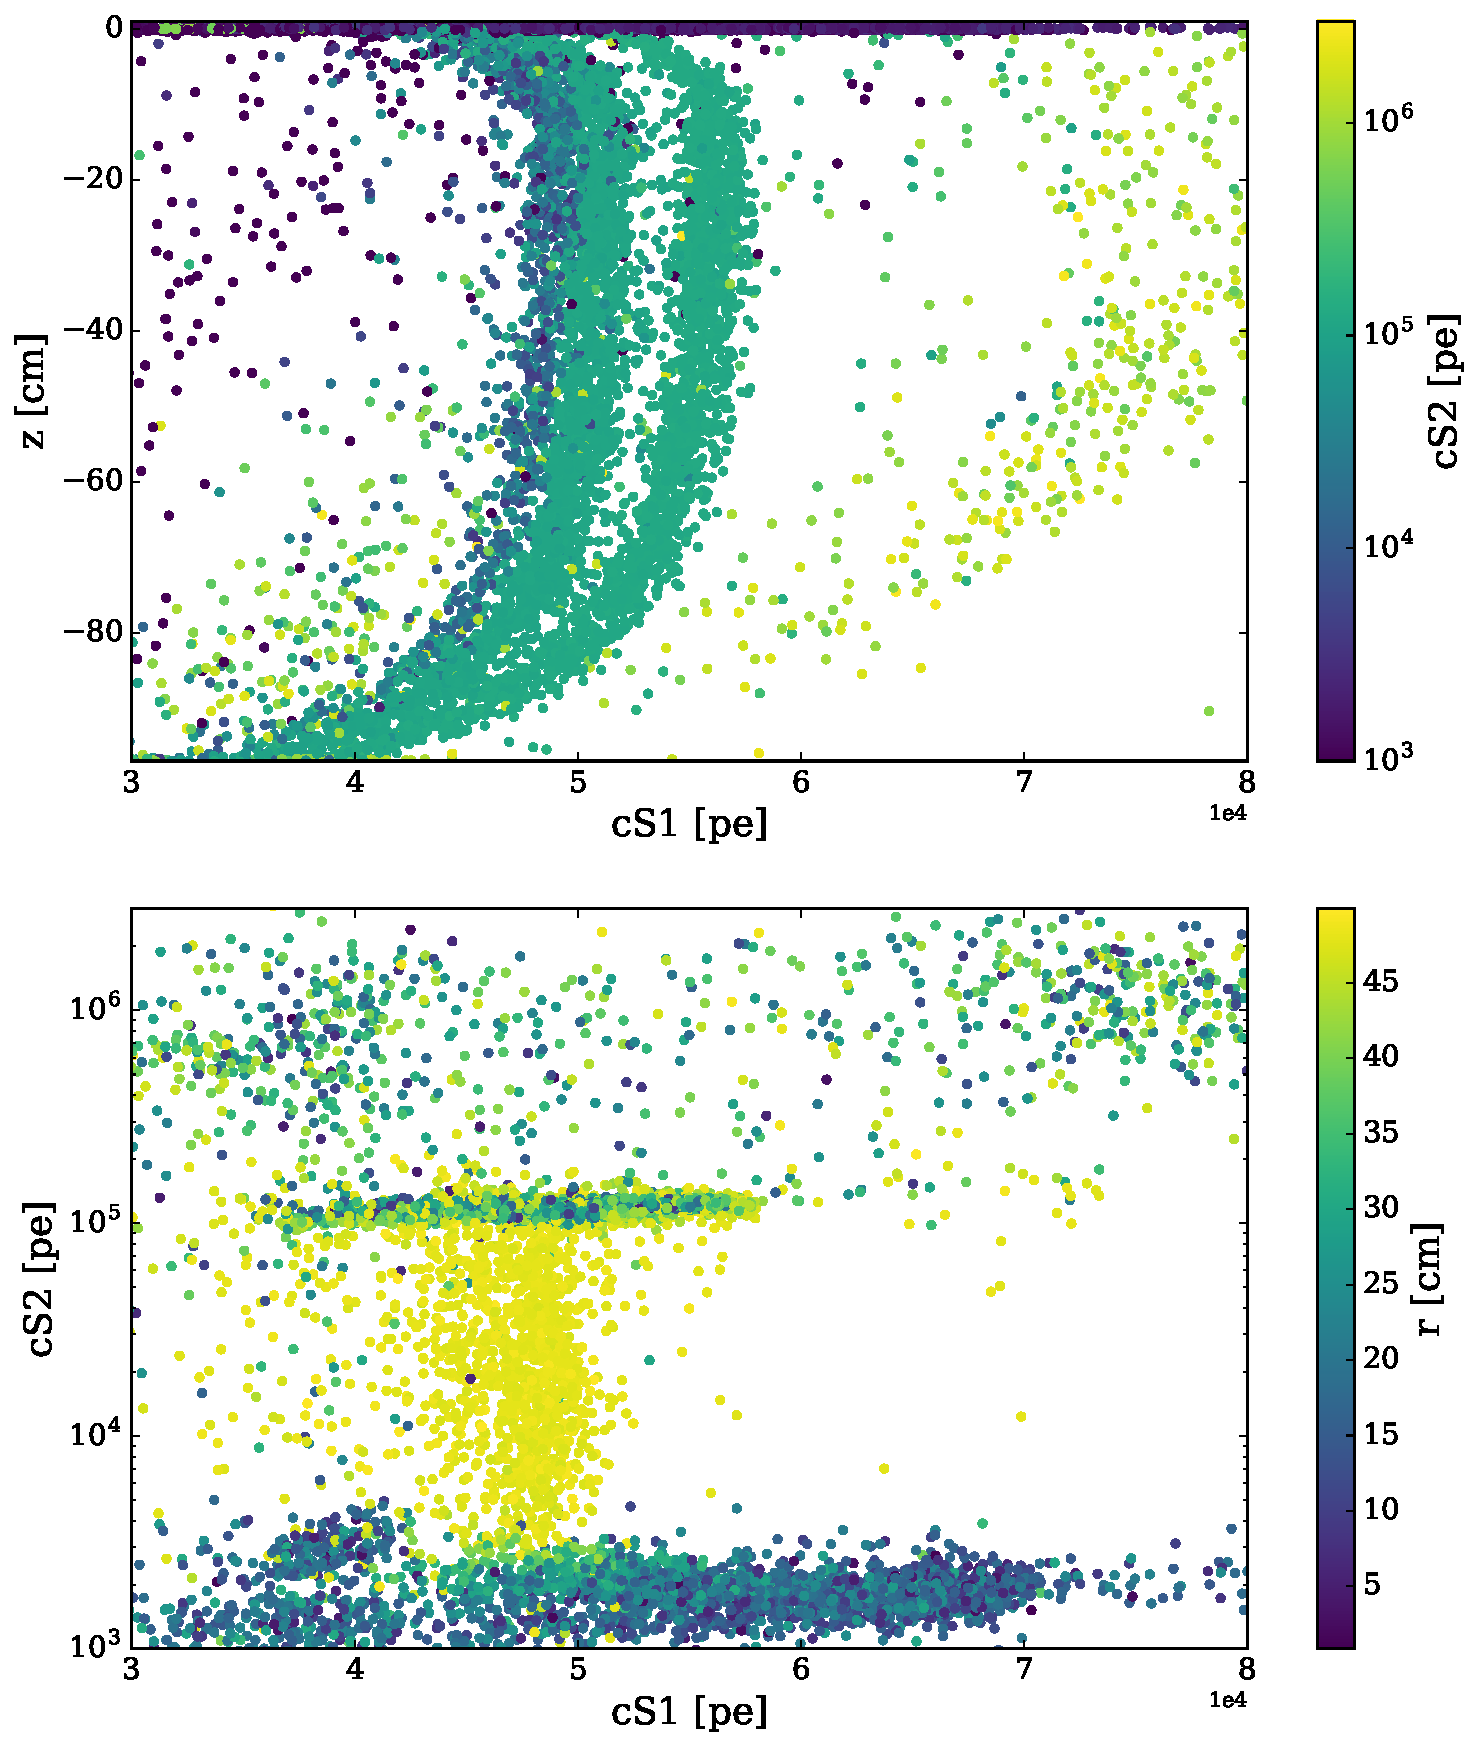
\includegraphics[width=0.8\textwidth]{figures/ml/ml_fig0}
    \caption{Alpha region of interest in XENON1T. (Left) The three populations are from decays of $^{210}$Po, \Rn, and \Po. The color of each point corrersponds to the reconstructed radial coordinate of the decay vertex, showing that \Rn~and \Po~events occupy the bulk while $^{210}$Po events occur at the edge of the detector. (Right) The $^{210}$Po events also suffer from poor charge collection, resulting in lower values of $cS2$. Machine learning techniques allow for the development of a cut that operates in multiple dimensions simultaneously, exploiting population separations otherwise difficult to see.}\label{fig:bulk_alphas}
\end{figure}

In this chapter, all ML algorithms are those available in the open-source scikit-learn package~\cite{skl} (SKL).

\section{Data formatting}

Most ML techniques require data to be scaled to a set range for the algorithms to function. One common scaling used is to set a mean of 0 and a standard deviation of 1, but for data that isn't normally distributed (like the data dealt with here) a better motivated scaling is over the $[0,1]$ range. For parameters that can vary by many orders of magnitude (for instance, $cS2$), the scaling can be based on the logarithm.

Also, it is important to decide which parameters of a dataset are useful for clustering. In XENON1T the full list of variables available to the analyst contains over 100 entries. While this can be used, it significantly increases the computational cost of the clustering, and often doesn't add any extra information useful for the algorithm to use. For instance, most analyses don't care about the minor differences between the results from the different position reconstruction methods. One method of dimensionality reduction is via Principle Component Analysis (PCA), which attempts to find the greatest variance from orthogonal combinations of variables. Alternately, variables can be manually chosen where there is a good motivation for separation.

For this analysis, the variables used are $cS1$, $cS2$, $s2_range_50p_area$ (width of the s2 signal that contains 50\% of the area, generally referred to as ``s2 width''), and $r_3d_nn$ and $z_3d_nn$ (positions reconstructed by the neural network, using the 3D position correction). These five variables are then scaled to lie in $[0,1]$, except for $cS2$ which is scaled so $\log cS2 \in [0,1]$, via the \texttt{MinMaxScaler} in the \texttt{preprocessing} module.

\section{Clustering}

SKL offers a variety of clustering algorithms, including:
\begin{itemize}
    \item \texttt{MiniBatchKMeans}
    \item \texttt{AffinityPropagation}
    \item \texttt{MeanShift}
    \item \texttt{SpectralClustering}
    \item \texttt{Ward}
    \item \texttt{AgglomerativeClustering}
    \item \texttt{DBSCAN}
    \item \texttt{Birch}
    \item \texttt{GaussianMixture}
\end{itemize}

Most algorithms are highly tunable, but the \texttt{GaussianMixture} method offers excellent out-of-the-box performance, very fast computation time. Others, like DBSCAN, take a lot of tweaking but can provide superior results. The Gaussian mixture takes, as an input, the desired number of clusters. It can take some tuning to find the best value for this; we take a value of 4. The value returned by the method is an array the same length as the input data, where each entry in the array is the cluster ID of the corresponding event. The populations themselves are largely constant if the clustering is redone, but the pouplation IDs often change. We show the results in various common groupings of parameters in Figure~\fig{fig:clustering}.

\begin{figure}[htbp]
    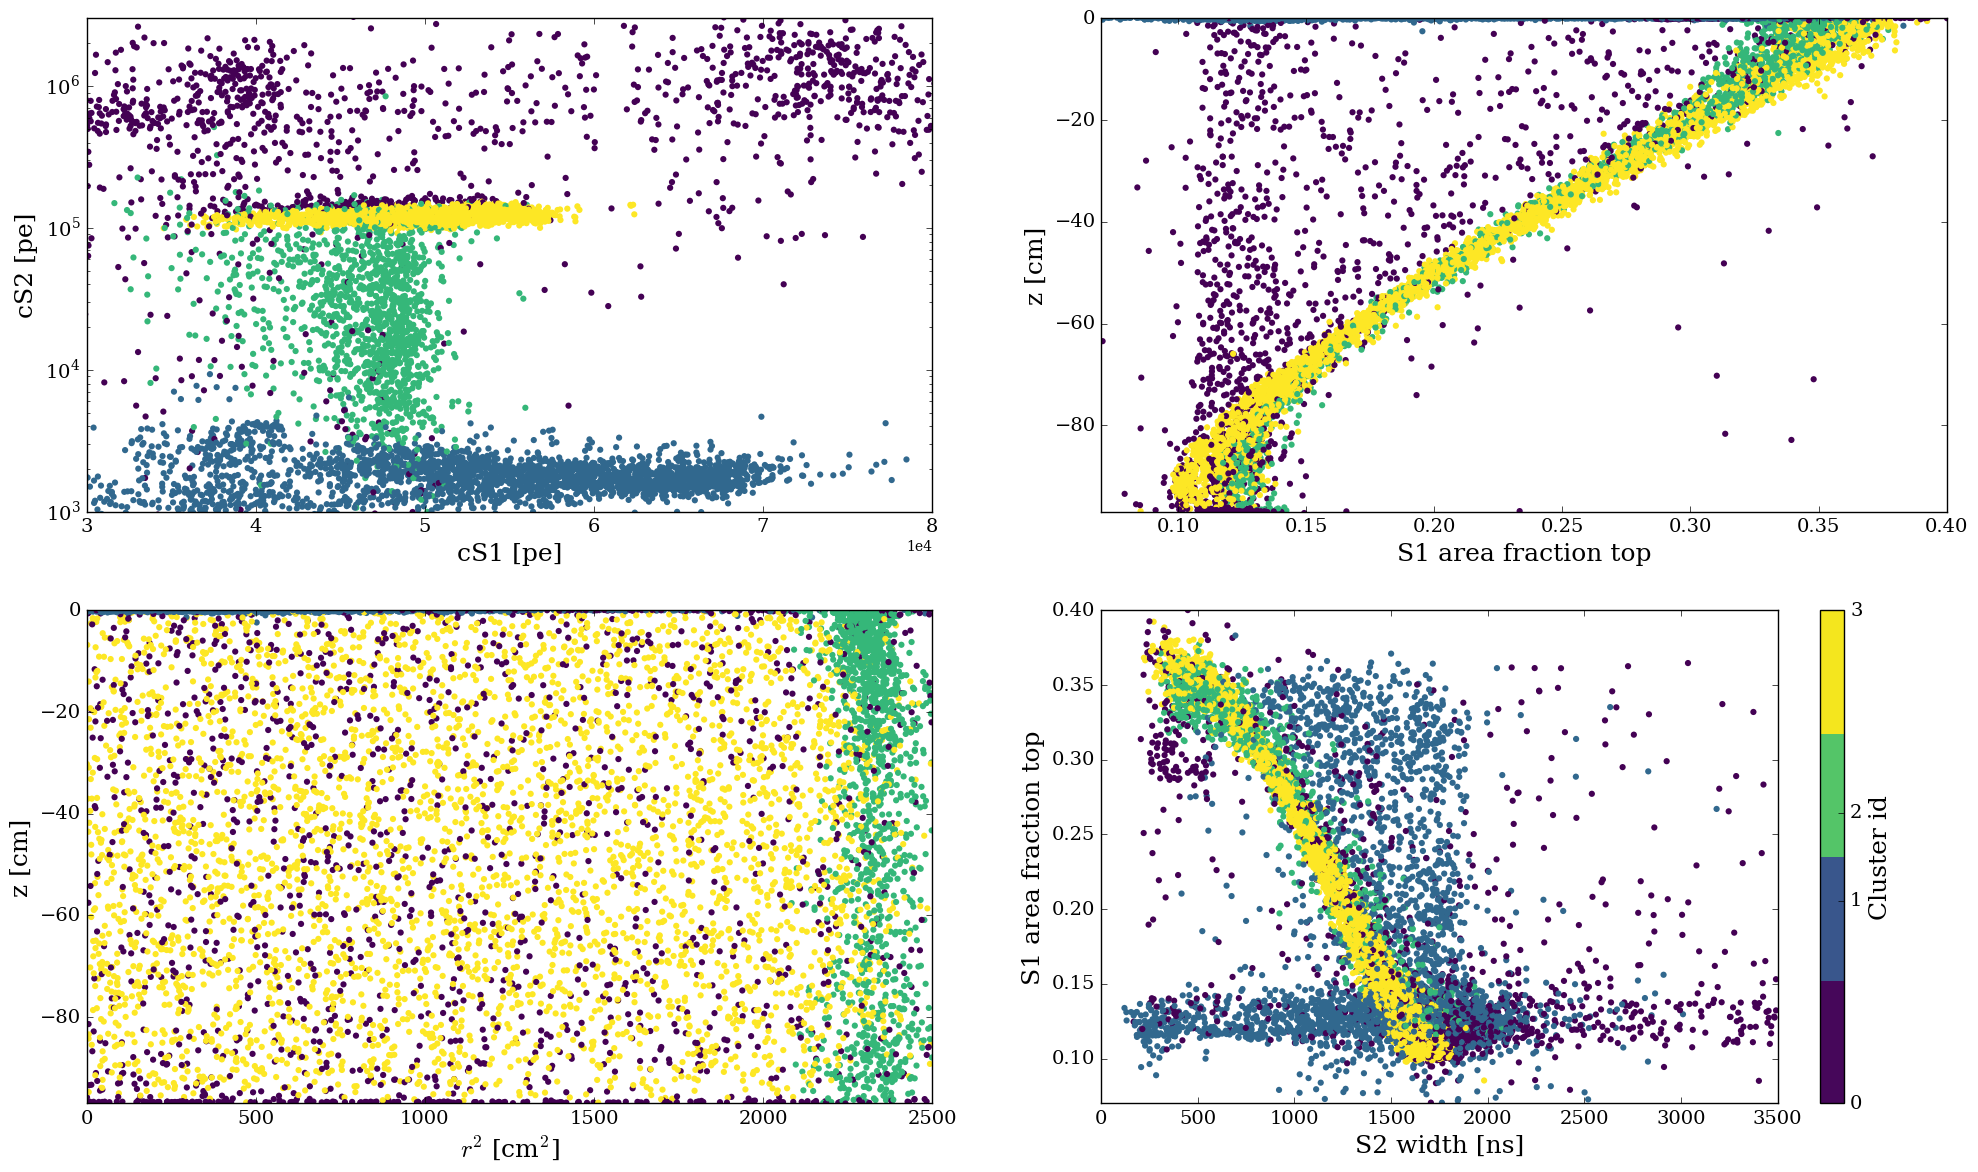
\includegraphics[width=\textwidth]{figures/ml/ml_clustering}
    \caption{Results from clustering in the alpha ROI, using the \texttt{GaussianMixture} method, displayed in common parameters. The color of each point indicates the cluster.}\label{fig:clustering}
\end{figure}

Once clustering is completed, the bulk alphas (green population) can be easily selected with their population ID. As this population includes both \Rn~and \Po, an additional step is necessary to separate them. For this population, the simplest method of separation is via a line between the two alpha lines in the $z-cS1$ parameter space, as shown in Figure~\ref{fig:split_alphas}. The \Rn~population is on the left of the line, and the \Po~population on the right. Some contamination is evident, but at a very low level.

\begin{figure}[htb]
    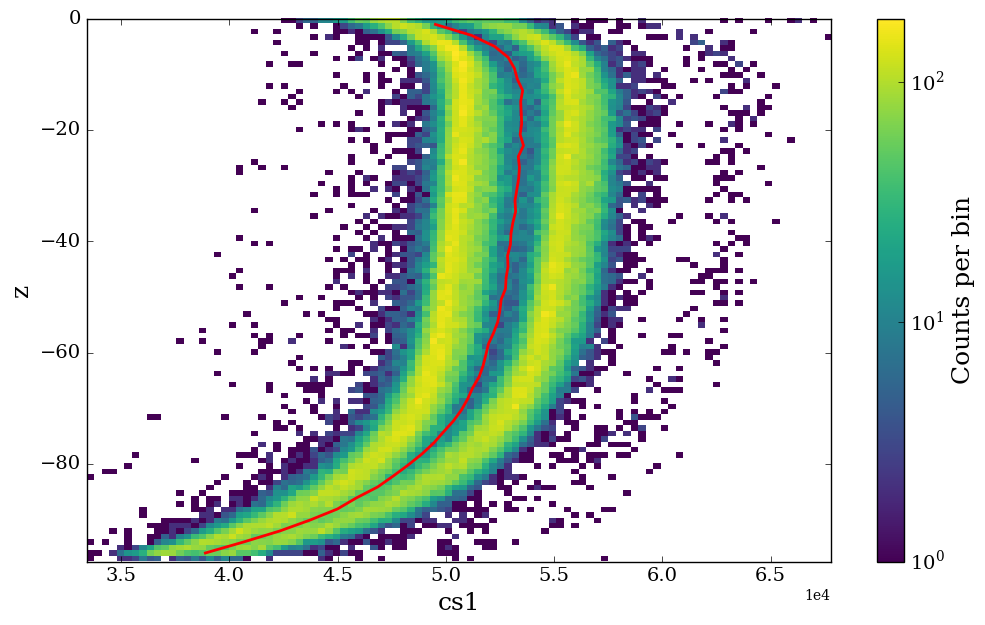
\includegraphics[width=0.8\textwidth]{figures/ml/ml_split_alphas}
    \caption{Once a clean selection of \Rn~and \Po~is in hand, separating them with a simple curve is straightforward.}\label{fig:split_alphas}
\end{figure}